\documentclass{beamer}
%\usepackage{amssymb}
%\usepackage{mathpazo}
\usepackage{multimedia}
%\usepackage{amsfonts}
%\usepackage{amsmath}
\usepackage{lscape}
\usepackage{scalefnt}
\usepackage{subfigure}
%\usepackage{stix}
%\usepackage{fdsymbol}
\usepackage{forloop}
\usepackage{color}
\usepackage{pgffor}
\usepackage{hyperref}
\usepackage[authoryear,round,longnamesfirst]{natbib}
\usepackage{tikz}
\definecolor{picton-blue}{HTML}{00b7ff}
\definecolor{violet-red}{HTML}{ff3881}
\definecolor{sun}{HTML}{ffaf18}
\definecolor{electric-violet}{HTML}{871EFF}

%% xcolor and define colors -------------------------
\usepackage{xcolor}

% https://www.viget.com/articles/color-contrast/
\definecolor{purple}{HTML}{5601A4}
\definecolor{navy}{HTML}{0D3D56}
\definecolor{ruby}{HTML}{9a2515}
\definecolor{alice}{HTML}{107895}
\definecolor{daisy}{HTML}{EBC944}
\definecolor{coral}{HTML}{F26D21}
\definecolor{kelly}{HTML}{829356}
\definecolor{cranberry}{HTML}{E64173}
\definecolor{jet}{HTML}{131516}
\definecolor{asher}{HTML}{555F61}
\definecolor{slate}{HTML}{314F4F}

% Mixtape Sessions
\definecolor{picton-blue}{HTML}{00b7ff}
\definecolor{violet-red}{HTML}{ff3881}
\definecolor{sun}{HTML}{ffaf18}
\definecolor{electric-violet}{HTML}{871EFF}

\newcommand\pictonBlue[1]{{\color{picton-blue}#1}}
\newcommand\sun[1]{{\color{sun}#1}}
\newcommand\electricViolet[1]{{\color{electric-violet}#1}}
\newcommand\violetRed[1]{{\color{violet-red}#1}}

\newcommand\bgPictonBlue[1]{{\colorbox{picton-blue!20!white}{#1}}}
\newcommand\bgSun[1]{{\colorbox{sun!20!white}{#1}}}
\newcommand\bgElectricViolet[1]{{\colorbox{electric-violet!20!white}{#1}}}
\newcommand\bgVioletRed[1]{{\colorbox{violet-red!20!white}{#1}}}

\def\code#1{\texttt{#1}}

% Main theme colors
\definecolor{accent}{HTML}{00b7ff}
\definecolor{accent2}{HTML}{871EFF}
\definecolor{gray100}{HTML}{f3f4f6}
\definecolor{gray800}{HTML}{1F292D}


% Beamer Options -------------------------------------

% Background
\setbeamercolor{background canvas}{bg = white}

% Change text margins
\setbeamersize{text margin left = 15pt, text margin right = 15pt} 

% \alert
\setbeamercolor{alerted text}{fg = accent2}

% Frame title
\setbeamercolor{frametitle}{bg = white, fg = jet}
\setbeamercolor{framesubtitle}{bg = white, fg = accent}
\setbeamerfont{framesubtitle}{size = \small, shape = \itshape}

% Block
\setbeamercolor{block title}{fg = white, bg = accent2}
\setbeamercolor{block body}{fg = gray800, bg = gray100}

% Title page
\setbeamercolor{title}{fg = gray800}
\setbeamercolor{subtitle}{fg = accent}

%% Custom \maketitle and \titlepage
\setbeamertemplate{title page}
{
    %\begin{centering}
        \vspace{20mm}
        {\Large \usebeamerfont{title}\usebeamercolor[fg]{title}\inserttitle}\\
        {\large \itshape \usebeamerfont{subtitle}\usebeamercolor[fg]{subtitle}\insertsubtitle}\\ \vspace{10mm}
        {\insertauthor}\\
        {\color{asher}\small{\insertdate}}\\
    %\end{centering}
}

% Table of Contents
\setbeamercolor{section in toc}{fg = accent!70!jet}
\setbeamercolor{subsection in toc}{fg = jet}

% Button 
\setbeamercolor{button}{bg = accent}

% Remove navigation symbols
\setbeamertemplate{navigation symbols}{}

% Table and Figure captions
\setbeamercolor{caption}{fg=jet!70!white}
\setbeamercolor{caption name}{fg=jet}
\setbeamerfont{caption name}{shape = \itshape}

% Bullet points

%% Fix spacing between items
\let\olditemize=\itemize 
\let\endolditemize=\enditemize 
\renewenvironment{itemize}{\vspace{0.25em}\olditemize \itemsep0.25em}{\endolditemize}

%% Fix left-margins
\settowidth{\leftmargini}{\usebeamertemplate{itemize item}}
\addtolength{\leftmargini}{\labelsep}

%% enumerate item color
\setbeamercolor{enumerate item}{fg = accent}
\setbeamerfont{enumerate item}{size = \small}
\setbeamertemplate{enumerate item}{\insertenumlabel.}

%% itemize
\setbeamercolor{itemize item}{fg = accent!70!white}
\setbeamerfont{itemize item}{size = \small}
\setbeamertemplate{itemize item}[circle]

%% right arrow for subitems
\setbeamercolor{itemize subitem}{fg = accent!60!white}
\setbeamerfont{itemize subitem}{size = \small}
\setbeamertemplate{itemize subitem}{$\rightarrow$}

\setbeamertemplate{itemize subsubitem}[square]
\setbeamercolor{itemize subsubitem}{fg = jet}
\setbeamerfont{itemize subsubitem}{size = \small}








% Links ----------------------------------------------

\usepackage{hyperref}
\hypersetup{
  colorlinks = true,
  linkcolor = accent2,
  filecolor = accent2,
  urlcolor = accent2,
  citecolor = accent2,
}


% Line spacing --------------------------------------
\usepackage{setspace}
\setstretch{1.35}


% \begin{columns} -----------------------------------
\usepackage{multicol}


% Fonts ---------------------------------------------
% Beamer Option to use custom fonts
\usefonttheme{professionalfonts}

% \usepackage[utopia, smallerops, varg]{newtxmath}
% \usepackage{utopia}
\usepackage[sfdefault,light]{roboto}

% Small adjustments to text kerning
\usepackage{microtype}



% Remove annoying over-full box warnings -----------
\vfuzz2pt 
\hfuzz2pt


% Table of Contents with Sections
\setbeamerfont{myTOC}{series=\bfseries, size=\Large}
\AtBeginSection[]{
        \frame{
            \frametitle{Roadmap}
            \tableofcontents[current]   
        }
    }


% Tables -------------------------------------------
% Tables too big
% \begin{adjustbox}{width = 1.2\textwidth, center}
\usepackage{adjustbox}
\usepackage{array}
\usepackage{threeparttable, booktabs, adjustbox}
    
% Fix \input with tables
% \input fails when \\ is at end of external .tex file
\makeatletter
\let\input\@@input
\makeatother

% Tables too narrow
% \begin{tabularx}{\linewidth}{cols}
% col-types: X - center, L - left, R -right
% Relative scale: >{\hsize=.8\hsize}X/L/R
\usepackage{tabularx}
\newcolumntype{L}{>{\raggedright\arraybackslash}X}
\newcolumntype{R}{>{\raggedleft\arraybackslash}X}
\newcolumntype{C}{>{\centering\arraybackslash}X}

% Figures

% \imageframe{img_name} -----------------------------
% from https://github.com/mattjetwell/cousteau
\newcommand{\imageframe}[1]{%
    \begin{frame}[plain]
        \begin{tikzpicture}[remember picture, overlay]
            \node[at = (current page.center), xshift = 0cm] (cover) {%
                \includegraphics[keepaspectratio, width=\paperwidth, height=\paperheight]{#1}
            };
        \end{tikzpicture}
    \end{frame}%
}

% subfigures
\usepackage{subfigure}


% Highlight slide -----------------------------------
% \begin{transitionframe} Text \end{transitionframe}
% from paulgp's beamer tips
\newenvironment{transitionframe}{
    \setbeamercolor{background canvas}{bg=accent!40!black}
    \begin{frame}\color{accent!10!white}\LARGE\centering
}{
    \end{frame}
}


% Table Highlighting --------------------------------
% Create top-left and bottom-right markets in tabular cells with a unique matching id and these commands will outline those cells
\usepackage[beamer,customcolors]{hf-tikz}
\usetikzlibrary{calc}
\usetikzlibrary{fit,shapes.misc}

% To set the hypothesis highlighting boxes red.
\newcommand\marktopleft[1]{%
    \tikz[overlay,remember picture] 
        \node (marker-#1-a) at (0,1.5ex) {};%
}
\newcommand\markbottomright[1]{%
    \tikz[overlay,remember picture] 
        \node (marker-#1-b) at (0,0) {};%
    \tikz[accent!80!jet, ultra thick, overlay, remember picture, inner sep=4pt]
        \node[draw, rectangle, fit=(marker-#1-a.center) (marker-#1-b.center)] {};%
}


% DAGS ----------------------------------------------
\usepackage{tikz}
\usetikzlibrary{shapes,decorations,arrows,calc,arrows.meta,fit,positioning}
% Tikz settings optimized for causal graphs.
\tikzset{
    -Latex,auto,node distance =1 cm and 1 cm,semithick,
    state/.style ={ellipse, draw, minimum width = 0.7 cm},
    point/.style = {circle, draw, inner sep=0.04cm,fill,node contents={}},
    bidirected/.style={Latex-Latex,dashed},
    el/.style = {inner sep=2pt, align=left, sloped}
}


% Beamer tricks -------------------------------------
% Make \pause work in align environments
\makeatletter
\renewrobustcmd{\beamer@@pause}[1][]{%
  \unless\ifmeasuring@%
  \ifblank{#1}%
    {\stepcounter{beamerpauses}}%
    {\setcounter{beamerpauses}{#1}}%
  \onslide<\value{beamerpauses}->\relax%
  \fi%
}
\makeatother


\setcounter{MaxMatrixCols}{10}

\newcommand\independent{\protect\mathpalette{\protect\independenT}{\perp}}
\def\independenT#1#2{\mathrel{\rlap{$#1#2$}\mkern2mu{#1#2}}}
\newcommand{\possessivecite}[1]{\citeauthor{#1}'s (\citeyear{#1})}
\newtheorem{parameter}[theorem]{Parameter of Interest}
\newtheorem{condition}[theorem]{Condition}
\newtheorem{assumption}[theorem]{Assumption}
\newenvironment{stepenumerate}{\begin{enumerate}[<+->]}{\end{enumerate}}
\newenvironment{stepitemize}{\begin{itemize}[<+->]}{\end{itemize} }
\newenvironment{stepenumeratewithalert}{\begin{enumerate}[<+-| alert@+>]}{\end{enumerate}}
\newenvironment{stepitemizewithalert}{\begin{itemize}[<+-| alert@+>]}{\end{itemize} }

\newcommand{\imageframe}[1]{%
    \begin{frame}[plain]
        \begin{tikzpicture}[remember picture, overlay]
            \node[at = (current page.center), xshift = 0cm] (cover) {%
                \includegraphics[keepaspectratio, width=\paperwidth, height=\paperheight]{#1}
            };
        \end{tikzpicture}
    \end{frame}%
}

\begin{document}

% \title{Mixtape Sessions: Causal Inference ft. Machine Learning}
% \subtitle{Day 1}
% \author{Brigham R. Frandsen}
% \date{October 28, 2022}
% \institute{BYU}
% \maketitle

\imageframe{figures/title.png}

\begin{frame}[t]{Allow me to introduce myself}
\begin{itemize}
\item<1-> Economics professor at Brigham Young University in Utah

\begin{onlyenv}<1>
\begin{figure}
\includegraphics<1>[scale=.09,clip,trim=10in 10in 8in 0in]{figures/muddybike}
\end{figure}
\end{onlyenv}

\item<2-> 4 biological kids, 3 foster daughters, most of whom can now run and mountain bike faster than me

\begin{onlyenv}<2>
\begin{figure}
\includegraphics<2>[scale=.45,clip,trim=1.25in .5in 0in 1in]{figures/kidslot}
\end{figure}
\end{onlyenv}

\item<3-> A big fan of causal inference in observational settings:
\begin{itemize}[<3->]
	\item Quasi-experimental evaluations of the effects of unions
	
	{\footnotesize{\color{gray}(Frandsen 2016, 2017, 2021; Chen, Frandsen, Grabowski, Town, Sojourner 2015)}}

	\item Distributional effects
	
	{\footnotesize{\color{gray}(Frandsen and Lefgren 2018, 2021; Frandsen, Froelich, Melly 2012)}}
\end{itemize}
\item<3-> And of exploring machine learning in applied economics:
\begin{itemize}[<3->]
	\item Teach Machine Learning for Economists at BYU
	\item Research on the power of ML in empirical strategies
	
	{\footnotesize{\color{gray}(Angrist and Frandsen 2022)}}
\end{itemize}
\end{itemize}
\end{frame}

\begin{frame}{Effects Ex Machina: Where we're going}
\begin{itemize}
\item[] \textbf{Machine Learning + Heterogeneous Treatment Effects}
\item Causality primer/review
\item Machine learning (ML) prediction primer/review
\item Heterogeneous treatment effects
	\begin{itemize}
		\item When they matter
		\item Conceptual framework
		\item Using ML to predict treatment effects:
		\item[] Random Causal Forests
		\item Python/R implementation
	\end{itemize}
\item[] (Prequel to this course: Machine Learning and Causal Inference)
\end{itemize}
\end{frame}

\newcounter{pn} 
\forloop{pn}{14}{\value{pn}<45}{
\begin{frame}{Potential outcomes and treatment effects}
\centering\includegraphics[width=1\textwidth,page=\value{pn}]{figures/slidepics}
\end{frame}
}

\begin{frame}{Basic causal inference summary}
\begin{itemize}
\item Target (for now!):
\[
ATE = E\left[Y_i\left(1\right)-Y_i\left(0\right)\right]=E\left[{\color{blue}\tau_i}\right]
\]
\item Key identifying assumption:
\[
\left(Y_i\left(0\right),Y_i\left(1\right)\right) \independent D_i | X_i
\]
\item Estimation:
	\begin{itemize}
		\item Multiple linear regression (OLS)
		\[
			Y_i = \beta_0 + \tau D_i +\beta_1 X_{1i} + \cdots + \beta_k X_{ki} +\varepsilon
		\]
		\item Matching
		\item Propensity score methods
		\item Machine-assisted:
		\begin{itemize}
			\item Post-Double Selection Lasso
			\item Double/De-biased Machine Learning
		\end{itemize}
	\end{itemize}
	\item Go to python!
\end{itemize}
\end{frame}

\begin{frame}[t]{Prediction Target}
\[
y_i = \alpha +\beta x_i + \varepsilon_i\vphantom{\underset{\hat{y}}{\underbrace{\alpha +\beta x_{i}}}}
\]
\includegraphics[scale=.5,clip,trim=2.5in 1.8in 1in .8in,page=45]{figures/slidepics}
\end{frame}

\begin{frame}[t]{Prediction Target}
\[
y_{i}={\color{picton-blue}\underset{\hat{y}}{\underbrace{\alpha +\beta x_{i}}}}+\varepsilon _{i}
\]
\includegraphics[scale=.5,clip,trim=2.5in 1.8in 1in .8in,page=46]{figures/slidepics}
\end{frame}

\begin{frame}[t]{Prediction  Methods}
Supervised machine learning algorithms:
\begin{itemize}
	\item Decision trees
	\item Random forests
	\item {\color{gray}Penalized regression (ridge, lasso)}
	\item {\color{gray}Support vector machines}
\end{itemize}
\end{frame}

\begin{frame}{Prediction mechanics}
\begin{columns}
\begin{column}{.4\textwidth}
\begin{itemize}
	\item<1-> \textbf{Goal:} Predict an out-of-sample outcome $Y$
	\item<2-> as a function, $\hat{f}\left(X\right)$, of \textbf{features} $X=\left(1,X_{1},X_{2},\dots,X_{K}\right)'$.
	\item<3-> Estimate the function $\hat{f}$ (aka ``train the model'') based on  \textbf{training sample} $\{(Y_i,X_i); i=1,...,N\}$
\end{itemize}
\end{column}
\begin{column}{.6\textwidth}
\begin{onlyenv}<1-3>
\includegraphics<1>[scale=.35,clip,trim=2.5in 1.8in 1in .8in,page=48]{figures/slidepics}
\includegraphics<2>[scale=.35,clip,trim=2.5in 1.8in 1in .8in,page=49]{figures/slidepics}
\includegraphics<3>[scale=.35,clip,trim=2.5in 1.8in 1in .8in,page=50]{figures/slidepics}
\end{onlyenv}
\end{column}
\end{columns}
\end{frame}

\begin{frame}{What's a ``good'' prediction?}
\begin{itemize}
	\item Want our prediction to be ``close,'' i.e. minimize the expected \textbf{mean squared error}:
	\[
		\min_{f(x)} E\left[\left(f\left(x\right)-Y\right)^2\middle|X=x\right]
	\]
\end{itemize}
\begin{center}
\includegraphics[scale=.35,clip,trim=2.5in 1.8in 1in .8in,page=52]{figures/slidepics}
\end{center}
\end{frame}

\foreach \x in {58,59,60,61} {
	\begin{frame}{Decision Trees}
		\includegraphics[scale=.5,clip,trim=2.5in .35in 0in 0in,page=\x]{figures/slidepics.pdf} 
	\end{frame}
}

\begin{frame}{Decision Trees}
\includegraphics[scale=.5,clip,trim=2.5in 3in 5.3in 2in,page=62]{figures/slidepics.pdf} 
\begin{itemize}
	\item Where to split:
	
	Choose the feature from $\left\{x_1,\ldots,x_p \right\}$ and the value of that feature to minimize MSE in the resulting child nodes
	\item Tuning parameters
	\begin{itemize}
		\item Max depth
		\item Min training obs per leaf
		\item Min improvement in fit in order to go ahead with a split
	\end{itemize}
\end{itemize}
\end{frame}
\begin{frame}{Forest for the Trees}
\begin{figure}
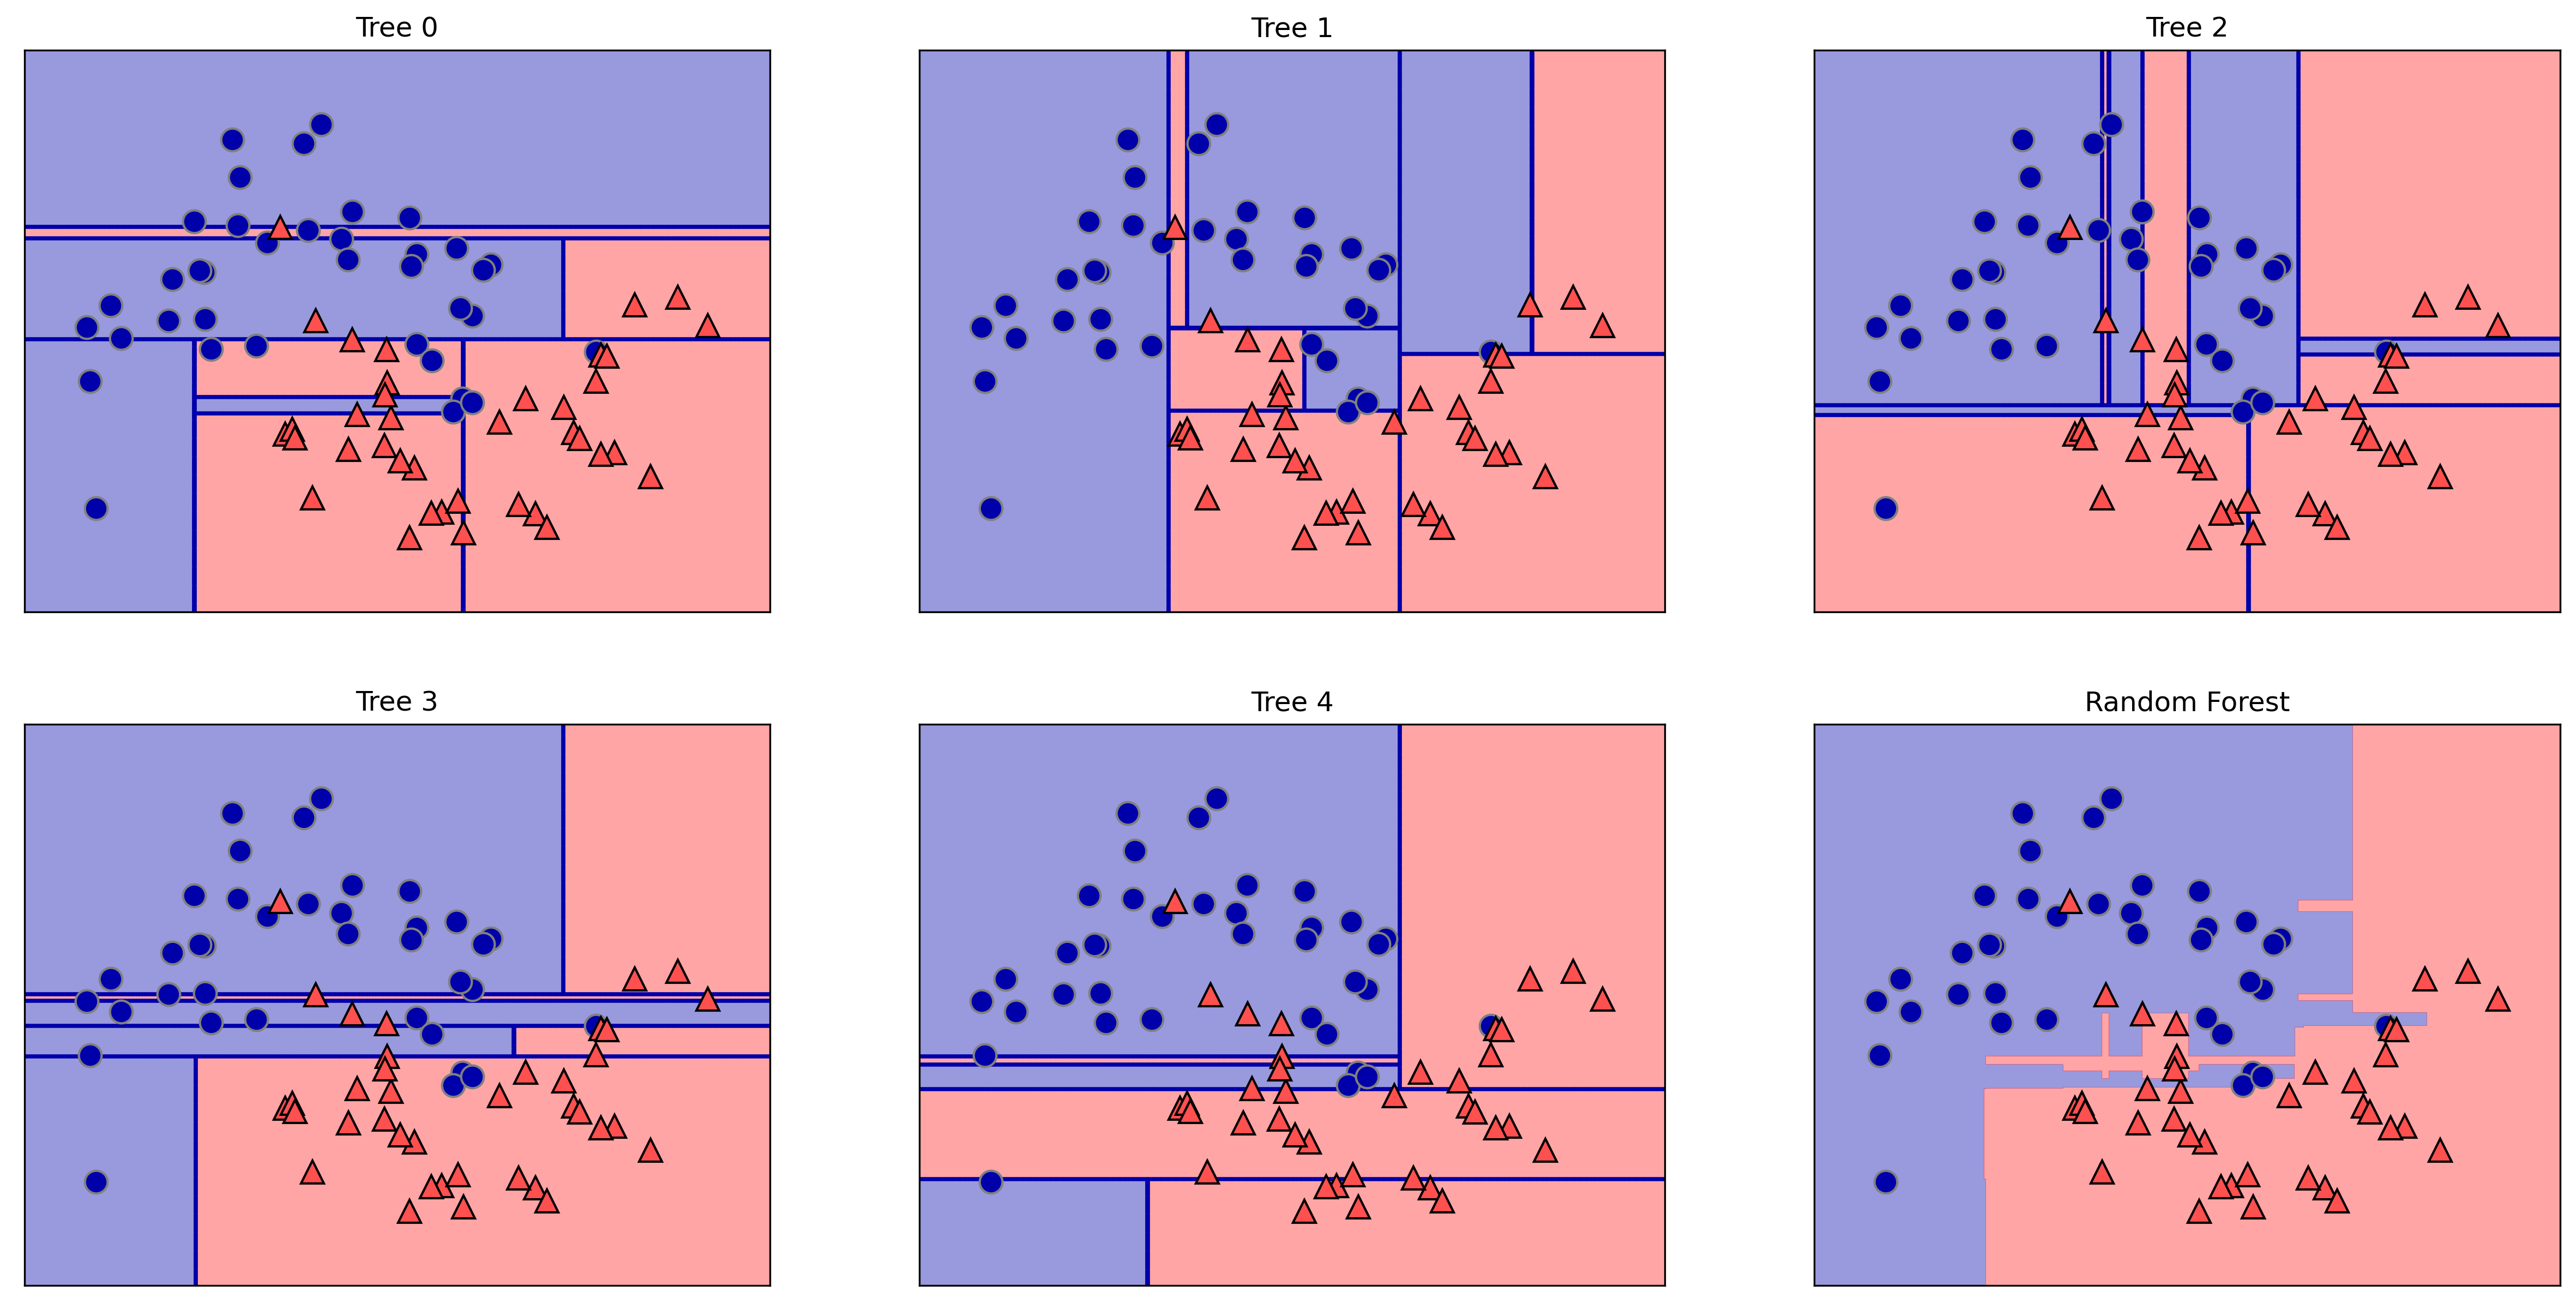
\includegraphics[scale=.2]{figures/randomforest}
\end{figure}
\begin{itemize}
	\item Value proposition: reduce variance by averaging together multiple predictions
	\item The catch: individual trees need to be \textbf{de-correlated}
	\item Algorithm:
	\begin{itemize}
		\item Grow $B$ trees, each on a different bootstrapped sample 
		\item At each split, consider only a random subset of features
		\item Average together the individual predictions
	\end{itemize}
	\item Let's grow some trees in python!
\end{itemize}
\end{frame}

\begin{frame}{Combining causal effects and ML: predicting heterogeneous treatment effects}
\begin{itemize}
	\item What is the effect of job training on the probability of finding a job . . .
\begin{itemize}
	\item for more-educated vs. less-educated individuals?
	\item for men vs. women?
	\item for married vs. single?
	\item for high-earning vs. low-earning (prior to training)?
	\item for minorities vs. non-minorities?
\end{itemize}
\item Why does it matter?
\item Other examples where heterogeneity in treatment effects matter?
\end{itemize}
\end{frame}

\begin{frame}{Traditional heterogeneity analysis: Interacted regression}
\begin{stepitemize}
\item[] To estimate the overall average effect:
\[
Y_i = \tau D_i + \varepsilon_i, \quad i\in\left\{1,\ldots,n\right\}
\]
\item[] To explore heterogeneity by sex:
\begin{eqnarray*}
Y_{i} &=&\tau ^{female}D_{i}+\varepsilon _{i},\qquad i:Female_{i}=1 \\
Y_{i} &=&\tau ^{male}D_{i}+\varepsilon _{i},\qquad i:Female_{i}=0,
\end{eqnarray*}%
\item[] or, equivalently:%
\begin{eqnarray*}
Y_{i} &=&\tau ^{male}D_{i}+\beta Female_{i}+\gamma D_{i}\times
Female_{i}+\varepsilon _{i}  \\
\tau ^{female} &=&\tau ^{male}+\gamma .
\end{eqnarray*}%
\item[] More generally,%
\begin{eqnarray*}
Y_{i} &=&\tau D_{i}+X_{i}^{\prime }\beta +D_{i}X_{i}^{\prime }\gamma
+\varepsilon _{i}, \\
\tau\left( x\right)  &=&\tau +x^{\prime }\gamma 
\end{eqnarray*}
\end{stepitemize}
\end{frame}

\begin{frame}{Challenges with traditional heterogeneity analysis}
\[
Y_{i} =\tau D_{i}+X_{i}^{\prime }\beta +D_{i}X_{i}^{\prime }\gamma
+\varepsilon _{i}
\]
\begin{itemize}
	\item Functional form: treatment effects may not vary linearly with $X_i$
	\item Curse of dimensionality: when $X_i$ includes many variables, OLS impractical or infeasible
	\item These are problems ML was born to solve!
\end{itemize}
\end{frame}

\begin{frame}{Predicting outcomes vs. treatment effects}
\begin{tabular}{p{2in}p{2in}}
Predicting outcomes & Predicting treatment effects \\ \hline
 & \\
Target: $\hat{y}\left(x\right) = E\left[Y_i|X_i=x\right]$ & Target: $\tau\left(x\right) = E\left[\tau_i|X_i=x\right]$\\ 
 & \\
Criterion: 
\[
\min E\left[\left(\hat{y}\left(x\right)-Y_i\right)^2|X_i=x\right] 
\]
& Criterion:
\[
\min E\left[\left(\tau\left(x\right)-\tau_i\right)^2|X_i=x\right] 
\]
\\
Training data: $\left\{Y_i,X_i\right\}_{i=1}^n$  & Training data: $\left\{{\color{red}\tau_i},X_i\right\}_{i=1}^n$ \\
\end{tabular}
\begin{stepitemize}
\item[]
\item[] Why is training data a problem for predicting treatment effecs?
\item Consequence: can't apply ML directly to predicting treatment effects; have to adapt them
\end{stepitemize}
\end{frame}

\begin{frame}{Adapting ML to predict treatment effects}
\begin{stepitemize}
	\item Break it up:
	\begin{eqnarray*}
	E\left[ \tau _{i}|X_{i}\right]  &:=&E\left[ Y_{i}\left( 1\right)
	-Y_{i}\left( 0\right) |X_{i}\right]  \\
	&=&E\left[ Y_{i}|X_{i},D_{i}=1\right] -E\left[ Y_{i}|X_{i},D_{i}=0\right] 
	\end{eqnarray*}
	(by what assumption?)
	\item Adjust the criterion: (why?)
	\[
		\min \sum_{i=1}^n\left(\tau\left(X_i\right)-\tau_i\right)^2 \iff \max \sum_{i=1}^n\tau\left(X_i\right)^2
	\]
	\item Be honest: use one set of observations to select the tree structure, and another to generate predictions
	\includegraphics[scale=.35,clip,trim=.25in 4in 3in .8in,page=63]{figures/slidepics}
\end{stepitemize}
\end{frame}

\begin{frame}{Predicting treatment effects using ML: Summary}
\begin{itemize}
\item Target: \[ CATE := \tau\left(x\right) = E\left[\tau_i|X_i=x\right] \]
\item Key identifying assumption: \[ \left(Y_i\left(0\right),Y_i\left(1\right)\right) \independent D_i | X_i \]
\item Estimation: Random Causal Forest
\begin{itemize}
	\item Grow decision trees on many bootstrapped samples
	\item Choose splits using the training set to $\max \sum_{i=1}^n\tau\left(X_i\right)^2$
	\item Generate predictions in each leaf using the estimation set
	\item Average predictions over the trees in the forest
\end{itemize}
\item Go to python!
\end{itemize}
\end{frame}
\begin{frame}
\huge Thank you!
\end{frame}

\end{document}
